\documentclass[12pt]{article}

\usepackage[margin=1in]{geometry} % 1-inch margins
\usepackage{times}                % Times (Times New Roman–like) font
\usepackage{fancyhdr}             % For custom headers/footers
\usepackage{setspace}             % For spacing
\usepackage{titlesec}             % For section formatting
\usepackage{enumitem}             % For list alignment
\usepackage{graphicx}             % For image insertion

\pagestyle{fancy}
\fancyhf{} % Clear default header and footer

% Header on the right side
\fancyhead[R]{Ultrasound Nerve Imaging And Clinical Decision Support System}

% Footer on the left side
\fancyfoot[L]{Pillai HOC College of Engineering \& Technology, Rasayani}
\fancyfoot[R]{\thepage} % Ensure page number is displayed on the right footer

% Horizontal lines in header & footer
\renewcommand{\headrulewidth}{0.4pt} 
\renewcommand{\footrulewidth}{0.4pt} 

% Set the page number to start from 25
\setcounter{page}{34}

\begin{document}

\vspace*{\fill}

\begin{center}
    {\Large \bf Chapter 6} \\[1em] % Line break with extra space (1em)
    {\Large \bf Project Design}
\end{center}
\vspace*{\fill}

\newpage

% Set section counter to 6 so that it starts as Chapter 6
\setcounter{section}{6}

\newpage

% SECTION 6.1: DATA FLOW DIAGRAM
\subsection{Data Flow Diagram}
\vspace{10pt}

A Data Flow Diagram (DFD) is a graphical representation that illustrates the flow of data through
a system, depicting processes, data sources, and interactions between entities. It helps in understanding how information moves through different components of the system.

\vspace{1em}

% SUBSECTION 6.1.1: DFD Level 0
\subsubsection{DFD Level 0}
\vspace{10pt}

\noindent DFD Level 0, also known as a Context Diagram, provides a high-level overview of the system,
showing how external entities interact with the system as a single unified process. It illustrates the
data flow from the user to the system, covering disease detection, prediction, and clinical decision-making.

\vspace{10pt}

\begin{center}
    \fbox{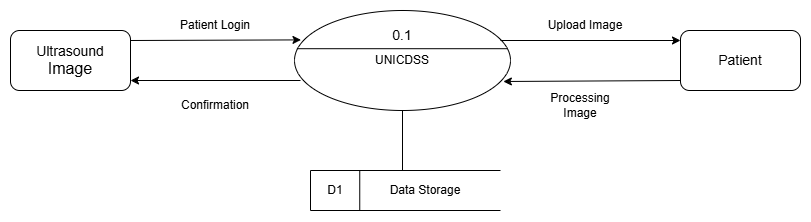
\includegraphics[width=1.0\textwidth]{DFD 0.drawio (2).png}}
\end{center}

\begin{center}
    \text{Figure 6.1.1 DFD Level 0}
\end{center}

\noindent The Level 0 Data Flow Diagram (DFD) for the Health Vision system provides a high-level overview of the system's primary functionalities and its interaction with external entities. At the center of the diagram is the main process labeled "0.1 Health Vision," which handles the core operations such as patient login, image upload, and data processing. The patient, as an external entity, initiates the interaction by logging into the system and uploading an ultrasound image. This image is then processed by the Health Vision system. The system communicates with a data storage unit (D1), where it retrieves or stores relevant data such as patient information and image results. Once the image is processed, confirmation is sent back to the ultrasound image entity, completing the flow. This high-level DFD highlights the essential flow of data between the user, the system, and its database, offering a simplified view of the system's overall functionality.
\vspace{20pt}
\newpage
% SUBSECTION 6.1.2: DFD Level 1
\subsubsection{DFD Level 1}
\vspace{10pt}

The Level 1 Data Flow Diagram (DFD) for the system provides a more detailed breakdown of
the system’s processes, depicting the steps involved in ultrasound image processing for disease
detection and clinical decision support. The process starts when the patient registers and logs in,
undergoing authentication through the credentials database (D2). After authentication, the patient
uploads an ultrasound image, which is stored and processed within the system and saved in multiple
databases (D3, D4, D6, D7, and D9). The system then applies Disease Segmentation, using AI
models to analyze the uploaded images and store segmented data in D5 (Image Data Storage).
Following this, Data Analysis is performed, where abnormalities are detected, and the Medical
Condition is identified. If an abnormality is found, Disease Detection is verified, and a detailed
analysis report is generated. The final report includes diagnostic results, suggested treatments, and
clinical guidance for the patient.

\vspace{10pt} 


\begin{center}
    \setlength{\fboxrule}{1pt}  % Border thickness
    \setlength{\fboxsep}{5pt} 
    \fbox{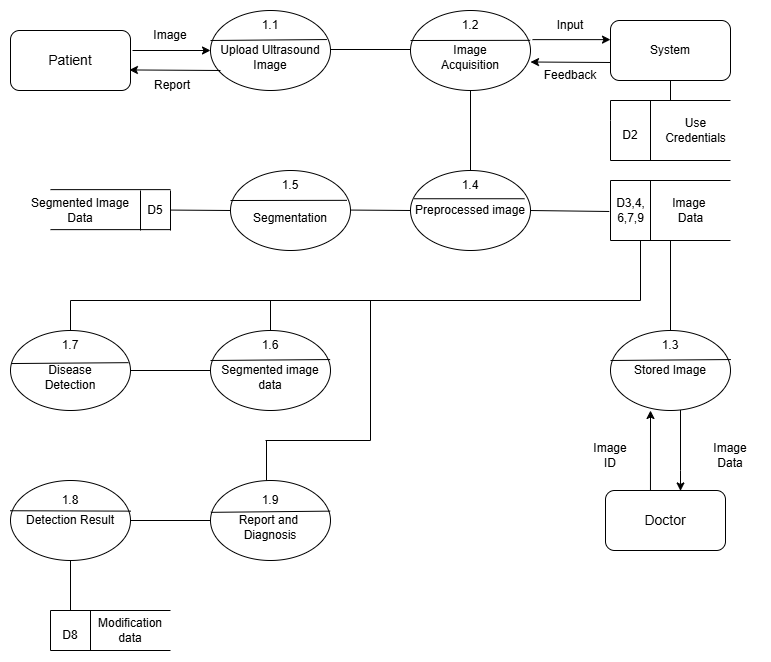
\includegraphics[width=1.0\textwidth, keepaspectratio]{DFDLevel1.drawio (2).png}}
\end{center}

\begin{center}
    \text {Figure 6.1.2 DFD Level 1}
\end{center}
\noindent The Level 1 Data Flow Diagram (DFD) for the Health Vision system provides a detailed breakdown of the internal processes involved in handling patient-submitted ultrasound images. The system begins with the patient providing input through the "Ultrasound Image" process (1.1), followed by image acquisition (1.2), which uses credentials stored in data store D2 for authentication. The acquired image is then preprocessed (1.4), and relevant image data is retrieved from data store D3.4, 6.7, and 7.9. The preprocessed image is stored (1.3) and associated with an Image ID, which is accessible to the patient. Simultaneously, the preprocessed image undergoes segmentation (1.5), generating segmented image data stored in D5. This data supports disease detection (1.7), leading to detection results (1.8) and a comprehensive report and diagnosis (1.9). The system also allows for modification of data (D8), ensuring adaptability. This diagram outlines the complete workflow from image input to diagnosis, highlighting how patient data is securely processed, stored, and analyzed within the system.
\newpage
% SECTION 6.2: FLOW CHART
\subsection{Flow Chart}

\vspace{10pt}

A flowchart is a step-by-step diagrammatic representation of a process that visually outlines the
sequence of actions within a system, showing decisions, inputs, and outputs in a structured manner.
In the Ultrasound-Based Clinical Decision Support System, the process begins when the patient
logs in and uploads an ultrasound image. The uploaded image undergoes preprocessing, where
noise is removed and quality enhancements are applied. Once preprocessing is complete, the
AI models, including CNN and YOLOv11, analyze the image to detect potential diseases. The
system generates a detailed report containing the detection results and medical recommendations if
a disease is identified. The patient then receives appropriate clinical guidance, including treatment
suggestions and next steps. If no abnormalities are detected, the system informs the patient that no
disease was found, and the process is completed. This flowchart ensures a systematic and efficient
approach to disease detection and clinical decision-making.
\newpage
\begin{figure}[h]
    \centering
    \fbox{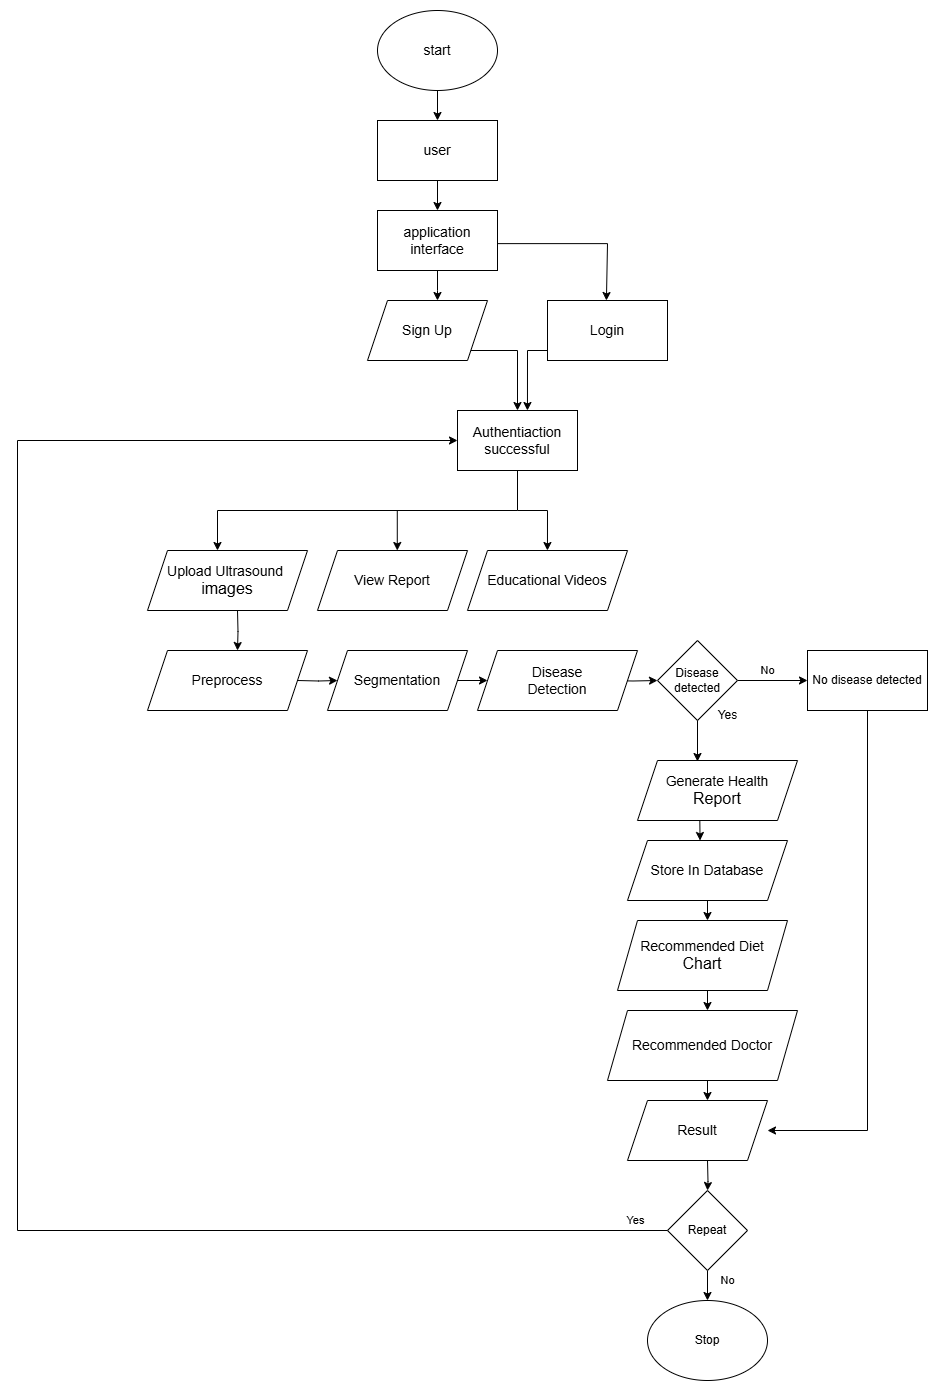
\includegraphics[width=0.8\textwidth]{flow update.drawio.png}}
    \renewcommand{\thefigure}{6.2.1} % Manual figure numbering
    \caption{Flow Chart Representation}
    \label{fig:flow_chart}
\end{figure}
\end{document}
